% SPDX-License-Identifier: CC-BY-SA-4.0
% Author: Matthieu Perrin
% Part: 
% Section: 
% Sub-section: 
% Frame: 

\begingroup

\begin{frame}{Transformation en forme normale de Chomsky}\label{slide:FNC}

  \begin{block}{Démonstration du théorème}
    Appliquer successivement les règles suivantes :
    \begin{enumerate}
    \item Introduire une règle \structure{$X \rightarrow x$} pour chaque $x\in \Sigma$
    \item Eliminer les règles \structure{$X \rightarrow ...S...$} 
    \item Eliminer les règles \structure{$X \rightarrow \varepsilon$} pour $X \not= S$
    \item Eliminer les règles \structure{$X \rightarrow Y$}
    \item Remplacer les règles \structure{$N \rightarrow A_1 A_2 ... A_n$} par \structure{$N \rightarrow A_1 B$} et \structure{$B \rightarrow A_2 ... A_n$}
    \end{enumerate}
  \end{block}

  \mode<beamer>{
  \begin{exampleblock}{Exemple}
    \scalebox{.9}{
      \begin{tikzpicture}
        \draw[white] (-2.5,1) rectangle (8.5,5);
        \draw (0,5) node[below]{\begin{minipage}{.45\textwidth}
            $\left\{
            \only<1>{\begin{array}{lll}
                S &\rightarrow& aSb \;|\; T \\
                T &\rightarrow& cT \;|\; \varepsilon\\
            \end{array}}
            \only<2>{\begin{array}{lll}
                S &\rightarrow& \alert{a}S\alert{b} \;|\; T \\
                T &\rightarrow& \alert{c}T \;|\; \varepsilon\\
            \end{array}}
            \only<3>{\begin{array}{lll}
                S &\rightarrow& A\alert{S}B \;|\; T \\
                T &\rightarrow& CT \;|\; \varepsilon\\
                A &\rightarrow& a  \\
                B &\rightarrow& b\\
                C &\rightarrow& c \\
            \end{array}}
            \only<4>{\begin{array}{lll}
                S &\rightarrow& D \\
                D &\rightarrow& ADB \;|\; T \\
                T &\rightarrow& CT \;|\; \alert{\varepsilon} \\
                A &\rightarrow& a \\
                B &\rightarrow& b \\
                C &\rightarrow& c \\
            \end{array}}
            \only<5>{\begin{array}{lll}
                S &\rightarrow& D \\
                D &\rightarrow& ADB \;|\; T \;|\; \alert{\varepsilon} \\
                T &\rightarrow& CT \;|\; C \\
                A &\rightarrow& a \\
                B &\rightarrow& b \\
                C &\rightarrow& c \\
            \end{array}}
            \only<6>{\begin{array}{lll}
                S &\rightarrow& \alert{D} \;|\; \varepsilon \\
                D &\rightarrow& ADB  \;|\; AB \;|\; \alert{T} \\
                T &\rightarrow& CT \;|\; \alert{C} \\
                A &\rightarrow& a \\
                B &\rightarrow& b \\
                C &\rightarrow& c \\
            \end{array}}
            \only<7>{\begin{array}{lll}
                S &\rightarrow& \alert{ADB}  \;|\; AB \;|\; CT \;|\; c \;|\; \varepsilon \\
                D &\rightarrow& \alert{ADB}  \;|\; AB \;|\; CT \;|\; c \\
                T &\rightarrow& CT \;|\; c \\
                A &\rightarrow& a \\
                B &\rightarrow& b \\
                C &\rightarrow& c \\
            \end{array}}
            \only<8>{\begin{array}{lll}
                S &\rightarrow& AE  \;|\; AB \;|\; CT \;|\; c \;|\; \varepsilon \\
                D &\rightarrow& AE  \;|\; AB \;|\; CT \;|\; c \\
                E &\rightarrow& DB \\
                T &\rightarrow& CT \;|\; c \\
                A &\rightarrow& a \\
                B &\rightarrow& b \\
                C &\rightarrow& c \\
            \end{array}}
            \right.$
        \end{minipage}};
        \draw (6.5,5) node[below]{\begin{minipage}{.58\textwidth}
            \only<2>{
              Application de la règle 1.
              \begin{enumerate}
              \item Introduire trois nouveaux non-terminaux\\ $A$, $B$ et $C$ 
              \item Introduire les règles
                \\$A \rightarrow a$, $B \rightarrow b$, $C \rightarrow c$
              \item Remplacer $a$ par $A$, $b$ par $B$ et $c$ par $C$
                %\item Remplacer les terminaux\\ $aSb$ par $ASB$ et $cT$ par $CT$
              \end{enumerate}
            }
            \only<3>{
              Application de la règle 2.
              \begin{enumerate}
              \item Introduire un nouveau non-terminal $D$ 
              \item Renommer $S$ en $D$
              \item Introduire une règle $S \rightarrow D$
              \end{enumerate}
            }
            \only<4>{
              Application de la règle 3.
              \begin{enumerate}
              \item Isoler $\varepsilon$ dans $T$ :\\
                $\begin{array}{lll}
                T &\rightarrow& T' \;|\; \varepsilon\\
                T' &\rightarrow& CT\\
              \end{array}$

              \item Remplacer $T$ par sa définition $T' \;|\; \varepsilon$
              \item Renommer $T'$ en $T$
              \end{enumerate}
            }
            \only<5>{
              Application de la règle 3 à nouveau.
              \begin{enumerate}
              \item Isoler $\varepsilon$ dans $D$ :\\
                $\begin{array}{lll}
                D &\rightarrow& D' \;|\; \varepsilon\\
                D' &\rightarrow& ABD\;|\; T\\
              \end{array}$

              \item Remplacer $D$ par sa définition $D' \;|\; \varepsilon$
              \item Renommer $D'$ en $D$
              \end{enumerate}
            }
            \only<6>{
              Application de la règle 4.
              \begin{enumerate}
              \item Remplacer $T \rightarrow C$ par $T \rightarrow c$
              \item Remplacer $D \rightarrow T$ par $D \rightarrow CT \;|\; c$
              \item Remplacer $S \rightarrow D$ par $S \rightarrow ADB  \;|\; AB \;|\; CT \;|\; c$
              \end{enumerate}
            }
            \only<7>{
              Application de la règle 5.
              \begin{enumerate}
              \item Remplacer $S \rightarrow ADB$ par :\\
                $\begin{array}{lll}
                S &\rightarrow& AE\\
                E &\rightarrow& BD\\
              \end{array}$
              \end{enumerate}
            }
        \end{minipage}};
    \end{tikzpicture}}
  \end{exampleblock}
  }

  \mode<handout>{
    \begin{exampleblock}{Exemple}
      \begin{minipage}{.45\textwidth}
        $\left\{
        \begin{array}{lll}
          S &\rightarrow& aSb \;|\; T \\
          T &\rightarrow& cT \;|\; \varepsilon\\
        \end{array}\right.$
      \end{minipage}
      $\Rightarrow$      
      \begin{minipage}{.45\textwidth}
        $\left\{
        \begin{array}{lll}
          S &\rightarrow& AE  \;|\; AB \;|\; CT \;|\; c \;|\; \varepsilon \\
          D &\rightarrow& AE  \;|\; AB \;|\; CT \;|\; c \\
          E &\rightarrow& DB \\
          T &\rightarrow& CT \;|\; c \\
          A &\rightarrow& a \\
          B &\rightarrow& b \\
          C &\rightarrow& c \\
        \end{array}
        \right.$
      \end{minipage}
    \end{exampleblock}
  }

  
\end{frame}

\endgroup
